\documentclass[journal,12pt,twocolumn]{IEEEtran}

\usepackage{setspace}
\usepackage{gensymb}
\singlespacing
\usepackage[cmex10]{amsmath}

\usepackage{amsthm}

\usepackage{mathrsfs}
\usepackage{txfonts}
\usepackage{stfloats}
\usepackage{bm}
\usepackage{cite}
\usepackage{cases}
\usepackage{subfig}
\usepackage{float}
\usepackage{longtable}
\usepackage{multirow}

\usepackage{enumitem}
\usepackage{mathtools}
\usepackage{steinmetz}
\usepackage{tikz}
\usepackage{circuitikz}
\usepackage{verbatim}
\usepackage{tfrupee}
\usepackage[breaklinks=true]{hyperref}
\usepackage{graphicx}
\usepackage{tkz-euclide}

\usetikzlibrary{calc,math}
\usepackage{listings}
    \usepackage{color}                                            %%
    \usepackage{array}                                            %%
    \usepackage{longtable}                                        %%
    \usepackage{calc}                                             %%
    \usepackage{multirow}                                         %%
    \usepackage{hhline}                                           %%
    \usepackage{ifthen}                                           %%
    \usepackage{lscape}     
\usepackage{multicol}
\usepackage{chngcntr}

\DeclareMathOperator*{\Res}{Res}

\renewcommand\thesection{\arabic{section}}
\renewcommand\thesubsection{\thesection.\arabic{subsection}}
\renewcommand\thesubsubsection{\thesubsection.\arabic{subsubsection}}

\renewcommand\thesectiondis{\arabic{section}}
\renewcommand\thesubsectiondis{\thesectiondis.\arabic{subsection}}
\renewcommand\thesubsubsectiondis{\thesubsectiondis.\arabic{subsubsection}}


\hyphenation{op-tical net-works semi-conduc-tor}
\def\inputGnumericTable{}                                 %%

\lstset{
%language=C,
frame=single, 
breaklines=true,
columns=fullflexible
}
\begin{document}


\newtheorem{theorem}{Theorem}[section]
\newtheorem{problem}{Problem}
\newtheorem{proposition}{Proposition}[section]
\newtheorem{lemma}{Lemma}[section]
\newtheorem{corollary}[theorem]{Corollary}
\newtheorem{example}{Example}[section]
\newtheorem{definition}[problem]{Definition}

\newcommand{\BEQA}{\begin{eqnarray}}
\newcommand{\EEQA}{\end{eqnarray}}
\newcommand{\define}{\stackrel{\triangle}{=}}
\bibliographystyle{IEEEtran}
\raggedbottom
\setlength{\parindent}{0pt}
\providecommand{\mbf}{\mathbf}
\providecommand{\pr}[1]{\ensuremath{\Pr\left(#1\right)}}
\providecommand{\qfunc}[1]{\ensuremath{Q\left(#1\right)}}
\providecommand{\sbrak}[1]{\ensuremath{{}\left[#1\right]}}
\providecommand{\lsbrak}[1]{\ensuremath{{}\left[#1\right.}}
\providecommand{\rsbrak}[1]{\ensuremath{{}\left.#1\right]}}
\providecommand{\brak}[1]{\ensuremath{\left(#1\right)}}
\providecommand{\lbrak}[1]{\ensuremath{\left(#1\right.}}
\providecommand{\rbrak}[1]{\ensuremath{\left.#1\right)}}
\providecommand{\cbrak}[1]{\ensuremath{\left\{#1\right\}}}
\providecommand{\lcbrak}[1]{\ensuremath{\left\{#1\right.}}
\providecommand{\rcbrak}[1]{\ensuremath{\left.#1\right\}}}
\theoremstyle{remark}
\newtheorem{rem}{Remark}
\newcommand{\sgn}{\mathop{\mathrm{sgn}}}
\providecommand{\abs}[1]{\left\vert#1\right\vert}
\providecommand{\res}[1]{\Res\displaylimits_{#1}} 
\providecommand{\norm}[1]{\left\lVert#1\right\rVert}
%\providecommand{\norm}[1]{\lVert#1\rVert}
\providecommand{\mtx}[1]{\mathbf{#1}}
\providecommand{\mean}[1]{E\left[ #1 \right]}
\providecommand{\fourier}{\overset{\mathcal{F}}{ \rightleftharpoons}}
%\providecommand{\hilbert}{\overset{\mathcal{H}}{ \rightleftharpoons}}
\providecommand{\system}{\overset{\mathcal{H}}{ \longleftrightarrow}}
	%\newcommand{\solution}[2]{\textbf{Solution:}{#1}}
\newcommand{\solution}{\noindent \textbf{Solution: }}
\newcommand{\cosec}{\,\text{cosec}\,}
\providecommand{\dec}[2]{\ensuremath{\overset{#1}{\underset{#2}{\gtrless}}}}
\newcommand{\myvec}[1]{\ensuremath{\begin{pmatrix}#1\end{pmatrix}}}
\newcommand{\mydet}[1]{\ensuremath{\begin{vmatrix}#1\end{vmatrix}}}
\numberwithin{equation}{subsection}
\makeatletter
\@addtoreset{figure}{problem}
\makeatother
\let\StandardTheFigure\thefigure
\let\vec\mathbf
\renewcommand{\thefigure}{\theproblem}
\def\putbox#1#2#3{\makebox[0in][l]{\makebox[#1][l]{}\raisebox{\baselineskip}[0in][0in]{\raisebox{#2}[0in][0in]{#3}}}}
     \def\rightbox#1{\makebox[0in][r]{#1}}
     \def\centbox#1{\makebox[0in]{#1}}
     \def\topbox#1{\raisebox{-\baselineskip}[0in][0in]{#1}}
     \def\midbox#1{\raisebox{-0.5\baselineskip}[0in][0in]{#1}}
\vspace{3cm}
\title{CBSE Maths 12, 2007}
%\author{Peri Priyanka$^{*}$
\author{Peri Priyanka
	\thanks{}
}
\maketitle
\newpage
\tableofcontents
\bigskip
\renewcommand{\thefigure}{\theenumi}
\renewcommand{\thetable}{\theenumi}
Download all python codes from 
\begin{lstlisting}
https://github.com/PeriPriyanka/cbsemathsquestions/2007/12/matrices/codes/solutions
\end{lstlisting}
%
Get latex-tikz codes from 
%
\begin{lstlisting}
https://github.com/PeriPriyanka/cbsemathsquestions/2007/12/matrices/solutions
\end{lstlisting}
\section{Boolean Algebra}
\renewcommand{\theequation}{\theenumi}
\begin{enumerate}[label=\thesection.\arabic*.,ref=\thesection.\theenumi]
\numberwithin{equation}{enumi}
\item Write the boolean expressions representing the following circuit and simplify the Boolean expression.
 \begin{figure}[H]
   \centering
   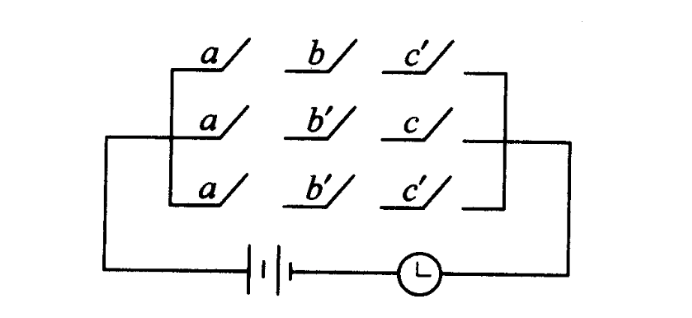
\includegraphics[width=1\columnwidth]{1.png}
   \caption{}
   \label{1}
\end{figure}
\solution\\
Truth table of the circuit \ref{1} is given in table \ref{table1}\\
\begin{table}[htb]
\tiny
 \resizebox{\columnwidth}{!}{ 
 \begin{tabular}{ |c|c|c|c| } 
 \hline
 a & b & c & out  \\
 \hline
0 & 0 & 0& 0\\
 \hline
 0 & 0 & 1& 0\\
 \hline
 0 & 1 & 0& 0\\
 \hline
 0 & 1 & 1& 0\\
 \hline
 1 & 0 & 0& 1\\
 \hline
 1 & 0 & 1& 1\\
 \hline
 1 & 1 & 0& 1\\
 \hline
 1 & 1 & 1& 0\\
 \hline
\end{tabular} }
 \caption{}
 \label{table1}
 \end{table}
 Therefore the  boolean expression representing the circuit \ref{1}
 \begin{align}
 out = ab'c'+ab'c+abc'
 \end{align} 

\item Show that the following argument is valid:
 \begin{align}
    & S_1 : p \vee q \nonumber \\
    & S_2 : \sim q \nonumber\\
    & S : p \wedge \sim q \nonumber
 \end{align}
 \solution\\
Truth table is shown in table \ref{table2} \\
\begin{table}[htb]
\tiny
 \resizebox{\columnwidth}{!}{ 
 \begin{tabular}{ |c|c|c|c|c| } 
 \hline
 p & q & $p \vee q$ & $\sim q$ & $p \wedge \sim q$  \\
 \hline
0 & 0 & 0& 1&0\\
 \hline
 0 & 1 & 1& 0&0\\
 \hline
 1 & 0 & 1& 1&1\\
 \hline
 1 & 1 & 1& 0&0\\
 \hline
\end{tabular} }
 \caption{}
 \label{table2}
 \end{table}
 Therefore from table \ref{table2} we can conclude that S is 1, if and only if $s_1$ and $s_2$ are 1.                                                                     
 \end{enumerate}
 \section{Algebra}
\renewcommand{\theequation}{\theenumi}
\begin{enumerate}[label=\thesection.\arabic*.,ref=\thesection.\theenumi]
\numberwithin{equation}{enumi}
\item  A particle starting with initial velocity of 30 m/sec moves with a uniform acceleration of 9 m/sec$^2$. Find :
\begin{enumerate}
   \item the velocity of the particle after 6 seconds.
   \item how far it will go in 9 seconds.
   \item its velocity when is has traversed 150 m.
\end{enumerate}
\solution\\
Given,
\begin{align}
& u = \text{initial velocity} =  30m/sec \\
& a = \text{acceleration} = 9 m/sec^2
\end{align}
\begin{enumerate}
\item
\begin{align} &v = u+at\\ & v =30+9(6) = 84 m/sec \end{align}
\item
\begin{align} &s=ut+\dfrac{1}{2}at^2\\ & s =30(9)+0.5(9)(9)^2 = 634.5m \end{align}
\item
\begin{align} &v = \sqrt{u^2 + 2as}\\ &v= \sqrt{900+2(9)(150)} = 60m/sec  \end{align}
\end{enumerate}
\item A ball projected with a velocity of 28 m/sec has a horizontal range 40 m. Find the two angles of projection.\\
\solution \\
Given,
\begin{align}
&R= \text{Range} = 40m\\
&u = \text{Initial velocity} = 28m/sec\\
&g = \text{acceleration due to gravity} =9.8m/sec^2
\end{align}
Let Angle of projection are $\theta$ and $90\degree-\theta$.
\begin{align}
&R = \dfrac{u^2\sin 2\theta}{g}\\
&\theta = \dfrac{1}{2}\sin^{-1}\left(\dfrac{Rg}{u^2}\right)\\
&\theta = 15\degree
\end{align}
Therefore angle of projection are 15\degree and 75\degree.
\item The resultant of two unlike parallel forces of 18 N and 10 N act along a line at a distance of 12 cm from the line of action of the smaller force. Find the distance between the lines of action of two forces.\\
\solution\\
Given, Two unlike forces 18N and 10N acting on a line. The distance of resultant from the smaller force 10N is 12cm and from 18N is x cm\\
Therefore,
\begin{align}
&18x = (12)(10)\\
&x = 6.66cm\\
\end{align}
The distance between two forces is 12+x = 18.66cm\\
\item Find the face value of a bill, discounted at 6\% per annum 146 days before the legal due date, if the banker's gain is Rs. 36.\\
\solution \\
Given,
\begin{table}[ht]
 \centering
 \resizebox{\columnwidth}{!}{
 \begin{tabular}{ |c|c|c| } 
 \hline
 Symbol & Description & Value\\
 \hline
G & Banker's gain  & 36 \\
 \hline
 D & Discount & 6\% per annum \\
 \hline
 n & Period of interest & 146 days \\
 \hline
 F & Face value & ? \\
 \hline
 \end{tabular}}
 \caption{}
 \end{table}
 \begin{align}
& F = G\left(1+\displaystyle\frac{Dn}{100}\right)\\
 & F =36\left(1+\displaystyle\frac{(6)(146)}{(100)(365)}\right)\\
 &F = 36.84
 \end{align}
 \item A bill for Rs. 7650 was drawn on 8th March 2005 at 7 months. It was discounted on 18 May 2005 and the holder of the bill received Rs. 7497. What rate of interest did the banker charge ?\\
 \solution\\
 Given,
\begin{table}[ht]
 \centering
 \resizebox{\columnwidth}{!}{
 \begin{tabular}{ |c|c|c| } 
 \hline
 Symbol & Description & Value\\
 \hline
G & Banker's gain  & 7497 \\
 \hline
 D & Discount & ? \\
 \hline
 n & Period of interest & 146 days \\
 \hline
 F & Face value & 7650 \\
 \hline
 \end{tabular}}
 \caption{}
 \end{table}
 \begin{align}
& I= \dfrac{F.D.n}{100}\\
 &7650-7497 = \dfrac{(7650)(D)(146)}{(100)(365)}\\
 &D = 5\%
 \end{align}
 \item A, B, C entered into a partnership investing Rs. 12000, Rs. 16000 and
Rs. 20000 respectively. A as working partner gets 10\% of the annual profit for
the same. After 5 months, B invested Rs. 2000 more while C withdrew Rs. 2000
after 8 months from the start of the business. Find the share of each in an
annual profit of Rs. 97,000.\\
\solution\\
Amount A invests per annum = 12000 x 12 = 1,44,000\\
Amount B invests per annum = 16000 x 5 + 18000 x 7 = 2,06,000\\
Amount C invests per annum = 20000 x 8 + 18000 x 4 = 2,32,000\\
Share of A \begin{align}\dfrac{10}{100}\text{x}97000 = 9,700\end{align}
Total left = 97000-9700 = 87,300\\
Share of B and C are in the ratio = 206000 : 232000 = 103:116\\
Share of B \begin{align}\dfrac{103}{219}\text{x}87300 = 41,031\end{align}
Share of C  \begin{align}\dfrac{116}{219}\text{x}87300 = 46,269\end{align}

\item Find the present value of an annuity due of Rs. 700 per annum payable at the
beginning of each year for 2 years allowing interest 6\% per annum, compounded
annually.[Take $(1.06)^{-1} = 0.943$]\\
\solution\\
Given,
\begin{table}[ht]
 \centering
 \resizebox{\columnwidth}{!}{
 \begin{tabular}{ |c|c|c| } 
 \hline
 Symbol & Description & Value\\
 \hline
P & Principal  & ? \\
 \hline
 R & Rate & 6\% \\
 \hline
 n & Period of interest & 2 years \\
 \hline
 T & Total & 700 \\
 \hline
 \end{tabular}}
 \caption{}
 \end{table}
 \begin{align}
 &T= P\left(1+\dfrac{R}{100}\right)\left(1+\dfrac{R}{100}\right)\\
 & P =\dfrac{700}{ \left(1+\dfrac{6}{100}\right)\left(1+\dfrac{6}{100}\right)}\\
 & P = 622.47
 \end{align}

 \item The total cost C(x), associated with the production and making x units of an item is given by
\begin{align}
   C(x) = 0.005x^3 - 0.02x^2 + 30x + 5000 \nonumber
\end{align}
Find:
\begin{enumerate}
\item the average cost function.
\item the average cost of output of 10 units.
\item the marginal cost function.
\item the marginal cost when 3 units are produced.
 \end{enumerate}
 \solution\\ Given,
 \begin{align}
   C(x) = 0.005x^3 - 0.02x^2 + 30x + 5000 
\end{align}
\begin{enumerate}
\item 
\begin{align}
& \text{average cost} = \dfrac{C(x)}{x} \\
&= 0.005x^2 - 0.02x + 30 +\dfrac{5000}{x}\\
&\text{average cost}|_{x=10} = 530.3
\end{align}
\item 
\begin{align}
& \text{marginal cost} = \dfrac{dC(x)}{dx} \\
&= 0.015x^2 - 0.04x + 30\\ 
&\text{marginal cost}|_{x=3} = 31.015
\end{align}
 \end{enumerate}
  \end{enumerate}
 \section{Calculus}
\renewcommand{\theequation}{\theenumi}
\begin{enumerate}[label=\thesection.\arabic*.,ref=\thesection.\theenumi]
\numberwithin{equation}{enumi}
\item Evaluate the following integral:
\begin{align}
 \int \displaystyle\frac{1+x^2}{1+x^4}\,dx \nonumber
\end{align}
\solution \\
\begin{align}
&\int \displaystyle\frac{1+x^2}{1+x^4}\,dx \\
& = \int \displaystyle\frac{\dfrac{1}{x^2}+1}{\dfrac{1}{x^2}+x^2}\,dx \\
& = \int \displaystyle\frac{\dfrac{1}{x^2}+1}{\left(x - \dfrac{1}{x}\right)^2+2}\,dx \label{1.1}
\end{align}
let $x - \dfrac{1}{x} = t$ then, $\dfrac{1}{x^2}+1 =dt$. substituting in \eqref{1.1}.
\begin{align}
& = \int \displaystyle\frac{1}{t^2+2}\, dt\\
& = \dfrac{1}{\sqrt{2}}\tan ^{-1}\left(\dfrac{t}{\sqrt{2}}\right)+c\\
& = \dfrac{1}{\sqrt{2}}\tan ^{-1}\left(\dfrac{x - \dfrac{1}{x}}{\sqrt{2}}\right)+c\\
& = \dfrac{1}{\sqrt{2}}\tan ^{-1}\left(\dfrac{x^2 - 1}{\sqrt{2}x}\right)+c
\end{align}
\item Solve the following differential equation:
\begin{align}
x \cos y dy=(xe^x\log x + e^x) dx\nonumber
\end{align}
\solution\\
\begin{align}
&x \cos y dy=(xe^x\log x + e^x) dx \\
&\cos y dy=\dfrac{(xe^x\log x + e^x)}{x} dx \\
& \int \cos y\, dy =  \int \dfrac{(xe^x\log x + e^x)}{x}\, dx \\
& \sin y = \int \left(\dfrac{xe^x\log x}{x} + \dfrac{e^x}{x}\right)\, dx \\
& \sin y = e^x\log x + \int \dfrac{e^x}{x}\, dx - \int \dfrac{e^x}{x}\, dx \\
&  \sin y = e^x\log x
\end{align}
\item Form the differential equations of the family of the curves $y = A\cos 2x + B\sin 2x$, where A and B are constants.\\
\solution\\
\begin{align}
& y = A\cos 2x + B\sin 2x \\
& \dfrac{dy}{dx} = -2A\sin 2x + 2B\cos 2x \\
& \dfrac{d^2y}{dx^2} = -4A\cos 2x -4B\sin 2x \\
& \dfrac{d^2y}{dx^2} = -4(A\cos 2x + B\sin 2x) \\
& \dfrac{d^2y}{dx^2} = -4y
\end{align}
\item Solve the following differential equation:
\begin{align}
   \displaystyle\frac{dy}{dx} + 2y = 6e^x \nonumber
\end{align}
\solution \\
\begin{align}
&\displaystyle\frac{dy}{dx} + 2y = 6e^x
\end{align}
Linear Differential Equation of form \begin{align} \displaystyle\frac{dy}{dx} + P(X)y = Q(x) \end{align}. The Integrating factor is defined as,
\begin{align}
& \text{IF} = e^{\int {P(x)}dx}\\
& \text{IF} =  e^{\int {2}dx}\\
& \text{IF} = e^{2x}
\end{align}
Solution is of the form,\\
\begin{align}
&y.IF = \int (Q(x).IF dx)\\
&y.e^{2x} = \int (6e^x.e^{2x}) dx \\
&y.e^{2x} = 2e^{3x}+c
\end{align}
\item Evaluate:
\begin{align}
   \int \cos 4x\cos 3x\, dx 
\end{align}
\solution \\
\begin{align}
&\int \cos 4x\cos 3x\, dx\\
&\int \cos(7x)+\cos(x)dx\\
&\dfrac{-\sin 7x}{7} + \dfrac{-\sin x}{1}
\end{align}
\item Using the properties of definite integrals, prove the following:
\begin{align}
 \int_{0}^{\pi} \displaystyle\frac{x\tan x}{\sec x\cosec x}\, dx = \displaystyle\frac{\pi^2}{4} \nonumber
\end{align}
\solution\\
\begin{align}
&I(x) = \int_{0}^{\pi} \displaystyle\frac{x\tan x}{\sec x\cosec x}\, dx \\
&I(\pi - x) =  \int_{0}^{\pi} \displaystyle\frac{(\pi - x )\tan (\pi-x)}{\sec (\pi-x)\cosec(\pi- x)}\, dx \\
&I(\pi - x) =  \int_{0}^{\pi} \displaystyle\frac{(\pi - x ) - \tan x)}{ - \sec (x)\cosec(x)}\, dx \\
&I(x) = I(\pi - x)\\
&2I = \int_{0}^{\pi} \displaystyle\frac{\tan x}{\sec x\cosec x}\, dx \\
&2I = \int_{0}^{\pi} \sin^2x\, dx \\
&2I = \int_{0}^{\pi} \displaystyle\frac{1-\cos2x}{2}\, dx \\
& 2I= \displaystyle\frac{\pi^2}{2}\\
& I = \displaystyle\frac{\pi^2}{4}
\end{align}
\item Evaluate: 
\begin{align}
    \int \displaystyle\frac{\sin x}{(1-\cos x)(2-\cos x)}\, dx \nonumber
    \end{align}
 \solution \\
 \begin{align}
 & \int \displaystyle\frac{\sin x}{(1-\cos x)(2-\cos x)}\, dx  \label{1.2}
 \end{align}
$ \cos x =t , \sin x=dt$, substituting in \eqref{1.2}
\begin{align}
&=\int \displaystyle\frac{dt}{(1-t)(2-t)} \\
&= \int \dfrac{1}{1-t}+\dfrac{-1}{2-t}\, dt \\
&= -\log{1-t}+\log{2-t} +c\\
&= \log{\dfrac{2-t}{1-t}} +c\\
&= \log{\dfrac{2-\cos x}{1-\cos x}} +c
\end{align}
\item Find the value of k if the function
\begin{align}
    f(x) =
   \left\{
\begin{array}{ll}
      kx^2, & x\geq 1 \\
      4, & x <  1 
\end{array} \right. 
\text{is continuous at x = 1} \nonumber
\end{align}
\solution \\
For continuity,
\begin{align}
& f(a) = f(x^-)|_a =  f(x^+)|_a  \label{1.3}\\
& f(1) = k(1)^2 = k\\
&f(1^-) = 4\\
&f(1^+) = k
\end{align}
From equation \eqref{1.3} we get k=4.
\begin{figure}[H]
   \centering
   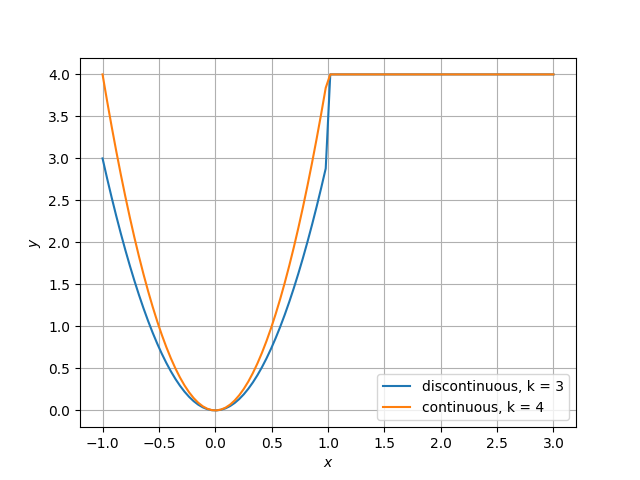
\includegraphics[width=1\columnwidth]{c_8.png}
   \caption{}
   \label{fig:1}
\end{figure}
\item Evalutate: 
 \begin{align}
    \lim_{x\to\frac{\pi}{4}} \left(\displaystyle\frac{\sin x - \cos x}{x - \displaystyle\frac{\pi}{4}}\right) \nonumber
 \end{align}
 \solution \\
 \begin{align}
& \lim_{x\to\frac{\pi}{4}} \left(\displaystyle\frac{\sin x - \cos x}{x - \displaystyle\frac{\pi}{4}}\right) \\
 &f\left(\dfrac{\pi}{4}^+\right) = \lim_{\delta \to 0} \left(\displaystyle\frac{\sin(\dfrac{\pi}{4}+\delta)  - \cos (\dfrac{\pi}{4}+\delta)}{\dfrac{\pi}{4}+\delta - \displaystyle\frac{\pi}{4}}\right)\\
 &f\left(\dfrac{\pi}{4}^+\right) = \lim_{\delta \to0} \left(\dfrac{\sqrt{2}\sin{\delta}}{\delta}\right)\\
 &f\left(\dfrac{\pi}{4}^+\right) = \sqrt{2}\\
 &f\left(\dfrac{\pi}{4}^-\right) = \lim_{\delta \to0} \left(\displaystyle\frac{\sin(\dfrac{\pi}{4}-\delta)  - \cos (\dfrac{\pi}{4}-\delta)}{\dfrac{\pi}{4}-\delta - \displaystyle\frac{\pi}{4}}\right)\\
 &f\left(\dfrac{\pi}{4}^-\right) = \lim_{\delta \to0} \left(-\dfrac{\sqrt{2}\sin{\delta}}{-\delta}\right)\\
 &f\left(\dfrac{\pi}{4}^-\right) = \sqrt{2}
 \end{align}
 For the limit to exist
 \begin{align}
 &f\left(\dfrac{\pi}{4}^+\right) = f\left(\dfrac{\pi}{4}^-\right) = \lim_{x\to\frac{\pi}{4}}f(x)
 \end{align}
 Therefore, \begin{align}\lim_{x\to\frac{\pi}{4}}f(x) = \sqrt{2}\end{align}
 \item Differentiate  $ \sin (x^2 + 1) $ with respect to x from first principle.\\
 \solution\\
 First principle of differentiation,
 \begin{align}
 &f'(x) = \lim_{h \to0}\dfrac{f(x+h)-f(x)}{h}\\
 & =  \lim_{h \to0} \dfrac{\sin((x+h)^2+1)-\sin (x^2+1)}{h}\\
 & =  \lim_{h \to0} \dfrac{\sin((x+h)^2+1)-\sin (x^2+1)}{h}\\
 & = \lim_{h \to0} 2\cos \left(\dfrac{2x^2+h^2+2xh+2}{2}\right).\dfrac{sin\left(\dfrac{h^2+2xh}{2}\right)}{h}\\
& = 2\cos \left(x^2 +1\right) \lim_{h \to0} \dfrac{\sin \left(\dfrac{h^2+2xh}{2}\right)}{h\left(\dfrac{h^2+2xh}{2}\right)} \left(\dfrac{h^2+2xh}{2}\right)\\
& = 2\cos \left(x^2 +1\right)
 \end{align}
 \item If y = $\sin(\log x)$, prove that
 \begin{align}
    & x^2\displaystyle\frac{d^2y}{dx^2} + x\displaystyle\frac{dy}{dx} + y = 0 \nonumber
 \end{align}
 \solution \\
 \begin{align}
    & x^2\displaystyle\frac{d^2y}{dx^2} + x\displaystyle\frac{dy}{dx} + y = 0 \label{21} \\
 & y = \sin(\log x)  \label{22}\\
 &\dfrac{dy}{dx} = \dfrac{\cos(\log x)}{x} \label{23}\\
 & \dfrac{d^2y}{dx^2} = \dfrac{-\sin(\log x)-\cos(\log x)}{x^2} \label{24}
 \end{align} 
 Substituting \eqref{22}, \eqref{23} and \eqref{24} in \eqref{21}.
 \begin{align}
 &= -\sin(\log x)-\cos(\log x)+\sin(\log x)+\cos(\log x)\\
 &= 0
 \end{align}
 \item Verify Rolle's theorem for the function $ f(x) = x^2-5x+4 $ on [1,4].\\
 \solution\\
 Rolle's theorem states that if a function f is continuous on the closed interval [a, b] and differentiable on the open interval (a, b) such that f(a) = f(b), then f'(x) = 0 for some $x \in a \leq x \leq b.$ \\
 Given,
 \begin{align}
 & f(x) = x^2-5x+4
 \end{align}
 \begin{enumerate}
 \item f(x) is continuous on [1, 4] being algebraic function.\\
 \item f'(x) =  2x-5 and differentiable on [1,4].\\
 \item 
 \begin{align}
 &f(a) = f(1) = (1)^2 -5(1)+4 = 0\\
 &f(b) = f(4) = (4)^2 -5(4) +4 =0 \\
 & f(a) = f(b)
 \end{align}
 \end{enumerate}
Rolle's is valid for f(x). Therefore f'(c) = 0\\
 \begin{align}
 &2c -5 = 0\\
 &c= 5/2
 \end{align}
 \item Evaluate $ \int_{0}^{2} (x^2+2x+1)\, dx $ as limit of sum. \\
 \solution\\
 Limit of the sum is defined as,
 \begin{align}
  \int_{a}^{b} f(x) dx=\lim_{h \to0}h[f(a)+f(a+h)+.+f(a+(n-1)h)] 
 \end{align}
 where,
 \begin{align}
& h= \dfrac{b-a}{n}\\
 & h = \dfrac{2}{n}\\
 &\int_{0}^{2} (x^2+2x+1)dx\\
 &= \lim_{h \to0}h[f(0)+f(h)+f(2h)+...+f((n-1)h)]\\
 & = \lim_{h \to0}h[1+...+((n-1)h)^2+2((n-1)h)+1]\\
 &=  \lim_{h \to0}h[n+...+((n-1)h)^2+2((n-1)h)+1]\\
&=  \lim_{h \to0}h[n+h^2(1^2+..+(n-1)^2+2h(1+..+(n-1)))]\\
& = \lim_{h \to0}h[n+h^2\left( \dfrac{n(n-1)(2n-1)}{6}\right) +2h \left( \dfrac{n(n-1)}{2}\right)
\end{align}
\begin{align}
& h\to 0; n\to \infty\\
& = \lim_{n \to\infty}\dfrac{2}{n}[n+\left(\dfrac{2}{n}^2\right)\left( \dfrac{n(n-1)(2n-1)}{6}\right) +2\left(\dfrac{2}{n}\right) \left( \dfrac{n(n-1)}{2}\right)\\
& =  \lim_{n \to\infty}[2+\dfrac{4}{3}(1-\dfrac{1}{n})(2-\dfrac{1}{n}) +4(1-\dfrac{1}{n})]\\
& = 2+4+\dfrac{8}{3} = \dfrac{26}{3} 
 \end{align}
 \end{enumerate}
 \section{Probability}
\renewcommand{\theequation}{\theenumi}
\begin{enumerate}[label=\thesection.\arabic*.,ref=\thesection.\theenumi]
\numberwithin{equation}{enumi}
\item An urn contains 7 red and 4 blue balls. Two balls are drawn at random with replacement. Find the probability of getting
\begin{enumerate}
\item 2 red balls
\item 2 blue balls
\item one red and one blue ball
\end{enumerate}
\solution\\
Let $X$ be a random variable such that $X \in\{0,1\}$.\\ $X$ represent type of ball.\\
All the red balls are mapped to $X=0$\\
 All the blue balls are mapped to $X=1$\\
 \begin{align}
&P(\text{Red}) =  P(X=0) = \dfrac{7}{11}\\
&P(\text{Blue}) =  P(X=1) = \dfrac{4}{11}
 \end{align}
 \begin{enumerate}
 \item 2 red balls
 \begin{align}
 P(X=0).P(X=0) = \dfrac{7}{11}.\dfrac{7}{11} =\dfrac{49}{121}
 \end{align}
 \item 2 blue balls
 \begin{align}
 P(X=1).P(X=1) = \dfrac{4}{11}.\dfrac{4}{11} =\dfrac{16}{121}
 \end{align}
 \item 1 red and 1 blue ball
 \begin{align}
 P(X=1).P(X=0) = \dfrac{4}{11}.\dfrac{7}{11} =\dfrac{28}{121}
 \end{align}
 \end{enumerate}
 \item A card is drawn at random from a well-shuffled pack of 52 cards. Find the probability that it is neither a ace nor a king.\\
 \solution\\
 Let $X$ be a random variable such that $X \in\{0,1\}$.\\ $X$ represent type of card.\\
Ace is mapped to $X=0$\\
 King is mapped to $X=1$\\
\begin{align}
&P(\text{Ace}) =  P(X=0) = \dfrac{4}{52} = \dfrac{1}{13}\\
&P(\text{King}) =  P(X=1) = \dfrac{4}{52} = \dfrac{1}{13} \\
&P(\overline{\text{Ace}}.\overline{ \text{king}}) = 1 - P(\text{Ace}+\text{king}) \\
&1 - P(\text{Ace}+\text{king}) = 1-P(X=0 + X=1)\\
&P(X=0 + X=1) = P(X=0)+ P(X=1) = \dfrac{2}{13} \\
&1-P(X=0 + X=1) = 1-\dfrac{2}{13} = \dfrac{11}{13}
 \end{align}
 \item There are two bags I and II. Bag I contains 2 white and 3 red balls and Bag II contains 4 white and 5 red balls. One ball is drawn at random from one of the bags and is found to be red. Find the probability that it was drawn from bag II.\\
 \solution\\
 Let $X$ be a random variable such that $X \in\{0,1\}$.\\ $X$ represent a Bag.\\
Bag1 is mapped to $X=0$\\
 Bag2 is mapped to $X=1$\\
Let $Y$ be a random variable such that $Y \in\{0,1\}$.\\ $Y$ represent type of Color.\\
All the red balls are mapped to $Y=0$\\
 All the white balls are mapped to $Y=1$\\
Given,
\begin{align}
&P(Bag1) = P(X=0) = \dfrac{1}{2}\\
&P(Bag2) = P(X=1) = \dfrac{1}{2}\\
&P\left(\dfrac{\text{Red}}{\text{Bag1}}\right) = P\left(\dfrac{Y=0}{X=0}\right) = \dfrac{3}{5}\\
&P\left(\dfrac{\text{White}}{\text{Bag1}}\right) = P\left(\dfrac{Y=1}{X=0}\right) = \dfrac{2}{5}\\
&P\left(\dfrac{\text{Red}}{\text{Bag2}}\right) = P\left(\dfrac{Y=0}{X=1}\right) = \dfrac{5}{9}\\
&P\left(\dfrac{\text{White}}{\text{Bag2}}\right) = P\left(\dfrac{Y=1}{X=1}\right) = \dfrac{4}{9}
\end{align}
Applying the Bayes theorem
\begin{align}
&P\left(\dfrac{\text{Bag2}}{\text{Red}}\right) = P\left(\dfrac{X=1}{Y=0}\right)\\
&P\left(\dfrac{X=1}{Y=0}\right) = \dfrac{P\left(\dfrac{Y=0}{X=1}\right).P(X=1)}{P\left(\dfrac{Y=0}{X=1}\right).P(X=1)+P\left(\dfrac{Y=0}{X=0}\right).P(X=0)}\\
& = \dfrac{\dfrac{5}{9}.\dfrac{1}{2}}{\dfrac{5}{9}.\dfrac{1}{2}+\dfrac{3}{5}.\dfrac{1}{2}}\\
& = \dfrac{25}{52}
\end{align}

\item Find the mean $\mu$, variance $\sigma^2$ for the following probability distribution:
\begin{table}[htb]
 \tiny
 \resizebox{\columnwidth}{!}{ 
 \begin{tabular}{ |c|c|c|c|c| } 
 \hline
 X & 0 & 1 & 2 & 3 \\
 \hline
P(X) & \(\frac{1}{8} \) & \(\frac{3}{8}\) & \(\frac{3}{8} \) & \(\frac{1}{8}\)\\
 \hline
\end{tabular} }
 \caption{}
 \end{table}\\
 \solution\\
 Mean or Expectation is defined as
 \begin{align}
 & E[X] = \Sigma_{i=0}^ \infty x_i p(X=x)
 \end{align}
 Mean square is defined as
 \begin{align}
 & E[X^2] = \Sigma_{i=0}^ \infty x_i^2 p(X=x)
 \end{align}
 Variance is defined as
 \begin{align}
 &var(X) =  E[X^2] -E[X]^2  
 \end{align}
 \begin{align}
 &E[X] = \Sigma_{i=0}^ \infty x_i p(X=x) \\
 & = 0.\dfrac{1}{8} +1.\dfrac{3}{8} +2.\dfrac{3}{8}+3.\dfrac{1}{8} \\
 & = \dfrac{3}{2}\\
 &E[X^2] = \Sigma_{i=0}^ \infty x_i^2 p(X=x) \\
 & = 0^2.\dfrac{1}{8} +1^2.\dfrac{3}{8} +2^2.\dfrac{3}{8}+3^2.\dfrac{1}{8} \\
 & = 3\\
 &var(X) =  E[X^2] -E[X]^2\\
 & = 3 - \left(\dfrac{3}{2}\right) \\
 & = \dfrac{3}{4}
 \end{align}
 \item Find the binomial distribution for which the mean is 4 and variance 3.\\
 \solution\\
 The PMF of Binomial distribution is defined as,
 \begin{align}
 & P(X=x) = \binom{n}{x}p^xq^{n-x}
 \end{align}
 Variance and Expectation of binomial distribution are given by,
 \begin{align}
 &E[X] =np\\
& var[X] = npq
 \end{align}
 Given,
 \begin{align}
 &E[X] =4\\
 &var[X] =3\\
 & q = \dfrac{npq}{np} = \dfrac{3}{4}\\
 & p =1-q = \dfrac{1}{4}\\
 &n = 16
 \end{align} 
 Therefore, the PMF is defined as
  \begin{align}
 & P(X=x) = \binom{16}{x}\dfrac{1}{4}^x\dfrac{3}{4}^{n-x}
 \end{align}
 \end{enumerate}
\section{Linear Algebra}
\renewcommand{\theequation}{\theenumi}
\begin{enumerate}[label=\thesection.\arabic*.,ref=\thesection.\theenumi]
\numberwithin{equation}{enumi}
\item
If $\vec{A} = \myvec{2&-3\\3&4}$, show that $ \vec{A}^2-6\vec{A}+17\vec{I}=0$. Hence find $\vec{A}^{-1}$. 
\solution Consider the matrix  given in the problem statement.
\begin{align}
&\vec{A} = \myvec{2&-3\\3&4}&
\end{align}
Considering the characteristic equation:  
\begin{align} 
& \vert\vec{A}-\lambda\vec{I}\vert = 0  & \label{eq:0.0.2}
\end{align}
From \eqref{eq:0.0.2} we get,
\begin{align}
&\begin{vmatrix}
  2-\lambda & -3\\ 3& 4-\lambda 
\end{vmatrix}
=0 \\
&(2-\lambda)(4-\lambda)+9=0\\ 
&\lambda^2-6\lambda+17=0 \label{eq:0.0.5} 
\end{align}
From the Cayley-Hamilton theorem \eqref{eq:0.0.5} can be written as
\begin{align}
&\vec{A}^2-6\vec{A}+17\vec{I} = 0  \label{eq:0.0.6} 
\end{align} 
Multiplying with $\vec{A}^{-1}$ on both sides of equation \eqref{eq:0.0.6}
We get,
\begin{align}
  &\vec{A}-6\vec{I}+17\vec{A}^{-1} = 0  \\
  &\vec{A}^{-1} = \displaystyle\frac{6\vec{I}-\vec{A}}{17} \\
  &\vec{A}^{-1} =  \myvec{4/17 &  3/17 \\ -3/17 & 2/17 }
\end{align}
\item Using the properties of determinants, prove the following:
\begin{center}
$\begin{vmatrix}
a-b-c & 2a& 2a\\ 2b& b-c-a& 2b\\2c&2c&c-a-b 
\end{vmatrix}$
$= (a+b+c)^3$
\end{center}
\solution
 \begin{align}
  &\begin{vmatrix}
    a-b-c & 2a& 2a\\ 2b& b-c-a& 2b\\2c&2c&c-a-b 
    \end{vmatrix}\\
& \xleftrightarrow[]{ R_1 \leftarrow R_1 + R_2+R_3}  \nonumber \\
&\begin{vmatrix} a+b+c & a+b+c& a+b+c \\ 2b& b-c-a& 2b\\2c&2c&c-a-b  \end{vmatrix}\\
  &= (a+b+c)\begin{vmatrix} 1 & 1 & 1\\ 2b& b-c-a& 2b\\2c&2c&c-a-b  \end{vmatrix}\\
   & \xleftrightarrow[]{ C_2 \leftarrow C_2- C_1 , C_3 \leftarrow C_3 - C_1} \nonumber \\
   &(a+b+c)\begin{vmatrix} 1 & 0 & 0\\ 2b& a+b+c& 0\\2c&0&a+b+c \end{vmatrix}\\
 &= (a+b+c)(a+b+c)^2  \\
 &= (a+b+c)^3 
  \end{align}
\item Using matrices, solve the following system of equation:
\begin{align}
   & x+2y-3z=6  \label{eq:0.0.16}  \\
   &  3x+2y-2z=3  \label{eq:0.0.17}\\
   &  2x-y+z=2   \label{eq:0.0.18}
\end{align}
\solution
Consider the equations given in the problem statement.
The solution can be found by solving the above system of linear equations.\\ 
System of linear equations are defined as 
\begin{align}
\vec{Ax=B} \label{eq:0.0.19}
\end{align}
From the equations \eqref{eq:0.0.16} ,\eqref{eq:0.0.17} and \eqref{eq:0.0.18}, 
\begin{align}
&\vec{A}= \myvec{1 &2 &-3\\3 & 2& -2\\2&-1&1} \\
\medskip
&\vec{x}= \myvec{ x\\ y\\z}\\
\medskip
&\vec{B}= \myvec{6\\3\\2}
\end{align} 
Substituting the values of $\vec{A}$, $\vec{x}$ and $\vec{B}$ in the equation \eqref{eq:0.0.19}
We get,
\begin{align}
&\myvec{1&2&-3\\3&2&-2\\2&-1&1} \myvec{x\\y\\z}= \myvec{6\\3\\2}
\end{align}
Considering the augmented matrix 
 \begin{align}
& \myvec{1&2&-3&6\\3&2&-2&3\\2&-1&1&2}
 \\
&\xleftrightarrow[]{ R_2 \leftarrow R_2 - 3R_1 , R_3 \leftarrow R_3 - 2R_1}
\myvec{1&2&-3&6\\0&-4&7&-15\\0&-5&7&-10}\\
 &\xleftrightarrow[]{ R_3 \leftarrow 4R_3 - 5R_2}
 \myvec{1&2&-3&6\\0&-4&7&-15\\0&0&-7&35}\\
 &\xleftrightarrow[]{ R_3 \leftarrow R_3/-7}
 \myvec{1&2&-3&6\\0&-4&7&-15\\0&0&1&-5}\\
 &\xleftrightarrow[]{ R_2 \leftarrow R_2-7R_3}
 \myvec{1&2&-3&6\\0&-4&0&20\\0&0&1&-5}\\
 &\xleftrightarrow[]{ R_2 \leftarrow R_2/-4}
 \myvec{1&2&-3&6\\0&1&0&-5\\0&0&1&-5}\\
 &\xleftrightarrow[]{ R_1 \leftarrow R_1-2R_2,R_1 \leftarrow R_1+3R_2}
 \myvec{1&0&-0&1\\0&1&0&-5\\0&0&1&-5}
 \end{align}
 \begin{align}
&\myvec{1&0&0\\0&1&0\\0&0&1} \myvec{x\\y\\z}= \myvec{1\\-5\\-5}& \label{eq:0.0.30}
\medskip
\end{align}
By solving equation \eqref{eq:0.0.30} we get,
\begin{align}
&x=1\\
&y= -5\\
&z=-5
\end{align}
Therefore, x=1, y= -5 and z=-5 are solutions to the given equations. 
\bigskip
\item Find the projection of $\overrightarrow{\vec{b}}+\overrightarrow{\vec{c}}$ on $\overrightarrow{\vec{a}}$ where $\overrightarrow{\vec{a}}=2\hat{\vec{i}}-2\hat{\vec{j}}+\hat{\vec{k}} , \overrightarrow{\vec{b}}=\hat{\vec{i}}+2\hat{\vec{j}}-2\hat{\vec{k}}$ and $ \overrightarrow{\vec{c}}=2\hat{\vec{i}}-\hat{\vec{j}}+4\hat{\vec{k}}$\\
\solution Consider the given vectors,
\begin{align}
&\vec{A}= \myvec{2\\-2\\1}\\
&\vec{B}=\myvec{1\\2\\-2}\\
&\vec{C}=\myvec{2\\-1\\4}
\end{align}
Projection of $\vec{(B+C)}$ on $\vec{A}$ is given by 
\begin{align}
&\displaystyle\frac{\vec{(B+C)}^\text T\vec{A}}{\|\vec{A}\|} \label{eq:0.0.38}
\end{align}
By substituting $\vec{A}$, $\vec{B}$ and $\vec{C} $ in \eqref{eq:0.0.38} we get, 
\begin{align}
  &\displaystyle\frac{\vec{(B+C)}^\text T\vec{A}}{\|\vec{A}\|}
&=\displaystyle\frac{\myvec{3&1&2}.\myvec{2\\-2\\1}}{\sqrt{4+4+1}} 
&=2 
\end{align}
\item Find the value of $\lambda$ which makes the vectors $\overrightarrow{\vec{a}}$,$\overrightarrow{\vec{b}}$ and $\overrightarrow{\vec{c}}$ coplanar, where $ \overrightarrow{\vec{a}}=2\hat{\vec{i}}-\hat{\vec{j}}+\hat{\vec{k}}$,$ \overrightarrow{\vec{b}}=\hat{\vec{i}}+2\hat{\vec{j}}-3\hat{\vec{k}}$ and $ \overrightarrow{\vec{c}}=3\hat{\vec{i}}-\lambda\hat{\vec{j}}+5\hat{\vec{k}}$\\
\solution Consider the given vectors,
\begin{align}
&\vec{A}= \myvec{2\\-1\\1}\\
&\vec{B}=\myvec{1\\2\\-3}\\
&\vec{C}=\myvec{3\\-\lambda\\5}
\end{align}
For the vectors $\vec{A}$, $\vec{B}$ and $\vec{C}$ to be coplanlar, the three vectors are linearly dependent. Therfore,
\begin{align}
  &\begin{vmatrix}
    2 & -1& 1\\ 1& 2& -3\\3&-\lambda&5 
    \end{vmatrix} = 0 \\
& = 2(10-3\lambda)+1(5+9)+1(-\lambda -6)=0\\
& \lambda=4
\end{align}
\item Find the equation of the plane which is perpendicular to the plane $5x + 3y + 6 z + 8 = 0$ and which contains the line of intersection of the planes $x + 2y + 3z - 4 = 0 $ and $2x + y - z + 5 = 0$.\\ 
\solution consider the given planes as
\begin{align}
&\vec{A}^\text T\vec{x}=\text c_1\nonumber \\&=\myvec{5&3&6}\myvec{x\\y\\z}=-8 \label{eq:0.0.46}\\ 
&\vec{B}^\text T\vec{x}=\text c_2\nonumber \\&=\myvec{1&2&3}\myvec{x\\y\\z}=4\\
  &\vec{C}^\text T\vec{x}=\text c_3\nonumber \\&=\myvec{2&1&-1}\myvec{x\\y\\z}=-5
\end{align}
Plane $\perp$ to $5x + 3y + 6 z + 8 = 0$ is given by,
\begin{align}
&(\vec{B}+\text k\vec{C})\vec{x}= \text c\\
&\left(\myvec{1\\2\\3}+\text k\myvec{2\\1\\-1}\right)^\text T.\myvec{x\\y\\z} =4-5\text k \label{eq:0.0.50} 
\end{align}
The plane in equation \eqref{eq:0.0.50} is $\perp$ to plane in equation \eqref{eq:0.0.46}. Therefore,
\begin{align}  
&\vec{A}^\text T. \left(\vec{B}+\text k\vec{C}\right) =0\\
&\myvec{5&3&6}.\left[\myvec{1\\2\\3}+\text k\myvec{2\\1\\-1}\right]=0\\
&\text k= \displaystyle\frac{-29}{7}
\end{align}
The required plane is \begin{align} \myvec{51&15&-50}\myvec{x\\y\\z}=-173 \end{align}
\item Find the resultant of two velocities 4 m/sec and 6 m/sec inclined to one another at an angle of 120\degree.\\
\solution\\
\begin{align}
& \vec{A} = \myvec{4\\0}\\
& \vec{B}= \myvec{6 \cos 120\degree\\6 \sin 120\degree } = \myvec{-3\\5.196} \\
& \text{Resultant} = \vec{A+B} = \myvec{1\\5.196}
\end{align}
\item A body of weight 70 N is suspended by two strings of length 27 cm and 36 cm, fastened to two points in the same horizontal line 45 cm apart and is in equilibrium. Find the tensions in the strings.\\
\solution\\
All the forces are shown in the figure.\\
Resolving the Tension along horizontal and vertical directions.\\
\begin{align}
&\cos \theta_1 = \sin \theta_2 = \dfrac{27}{45} \\
&\cos \theta_2 = \sin \theta_1 = \dfrac{36}{45}
\end{align}
Equating the Horizontal forces
\begin{align}
T_1\cos \theta_1 - T_2\cos \theta_2 =0
\end{align}
Equating the Vertical forces
\begin{align}
T_1\sin \theta_1 + T_2\sin \theta_2 = W
\end{align}
Putting in a matrix form
\begin{align}
&\myvec{\cos \theta_1& - \cos \theta_2\\ \sin \theta_1 & \sin \theta_2  }\myvec{T_1\\T_2} =\myvec{W\\0}\\
&\myvec{\dfrac{27}{45}& - \dfrac{36}{45}\\ \\ \dfrac{36}{45} & \dfrac{27}{45} }\myvec{T_1\\T_2} =\myvec{70\\0} \label{28}
\end{align}
Solving the  system of linear equations in \eqref{28} we get,
\begin{align}
\myvec{T_1\\T_2} = \myvec{57.71\\-44.21}
\end{align}
\end{enumerate}
\section{Optimization}
\renewcommand{\theequation}{\theenumi}
\begin{enumerate}[label=\thesection.\arabic*.,ref=\thesection.\theenumi]
\numberwithin{equation}{enumi}
\item Find the point on the curve $x^2=8y $ which is nearest to the point (2,4).\\
\solution\\
Given point, 
\begin{align}
&\vec{p} = \myvec{2\\4}
\end{align}
Forming an optimisation problem,\\
Variable of optimisation
\begin{align}
\vec{x} = \myvec{x\\y}
\end{align}
Objective function is defined as,
\begin{align}
Z = \min_{\vec{x}}\|\vec{x} - \vec{p}\|
\end{align}
Constraints
\begin{align}
&\vec{x}^T\vec{A}\vec{x}+2\vec{b}^T\vec{x}+c=0\\
&\vec{A} = \myvec{1&0\\0&0}\\
&\vec{b}= \myvec{-1/2\\0}\\
&c=0
\end{align}
The problem can be reframed as
\begin{align}
&Z = \min_{\vec{x}}\|\vec{x} - \vec{p}\| \nonumber\\
&\textrm{s.t.} \quad \vec{x}^T\vec{A}\vec{x}+2\vec{b}^T\vec{x}+c=0
\end{align}
\item Show that a right circular cylinder of least curved surface and given volume 125 $cm^3$ has an altitude equal to $ \sqrt{2} $ times the radius of the base.\\
\solution\\
Given,
\begin{table}[ht]
 \centering
 \resizebox{\columnwidth}{!}{
 \begin{tabular}{ |c|c| } 
 \hline
 Symbol & Description \\
 \hline
$r$ & radius of cylinder  \\
 \hline
 $h$ & height of cylinder \\
 \hline
 $s$ & surface area \\
 \hline
  $v$ & volume \\
 \hline
\end{tabular}}
 \caption{}
 \end{table}
 \begin{align}
 &s = \pi r h \\
 &v = \pi r^2h
 \end{align}
Framing as an optimization problem\\
\begin{align}
\min_{r,h} \quad &s \nonumber\\
\textrm{s.t.} \quad & 125= \pi r^2h\nonumber\\
  &h = \sqrt{2}r    
\end{align}
By solving in cvxpy we get the minimum surface area as $41cm^2$
\item If a young man rides his motorcycle at 25 km/hour, he had to spend Rs. 2 per
km on petrol. If he rides at a faster speed of 40 km/hour, the petrol cost increases
at Rs. 5 per km. He has Rs. 100 to spend on petrol and wishes to find what is
the maximum distance he can travel within one hour. Express this as an LPP.\\
\solution\\
Let us assume that the man travels x km when the speed is 25 km/hour and y km when the speed is 40 km/hour.\\
Thus, the total distance travelled is given by
\begin{align}
z = (x + y) km
\end{align}
Now, it is given that the man has Rs 100 to spend on petrol.\\
\begin{align}
\text{total cost }= 2x + 5y \leq 100
\end{align}
Now, time taken to travel x km = $\dfrac{x}{25}hrs$\\

Time taken to travel y km = $\dfrac{y}{40}hrs$\\

Now, it is given that the maximum time is 1 hour. So, we have
\begin{align}
&\dfrac{x}{25}+\dfrac{y}{40}\leq 1\\
&8x+5y\leq200
\end{align}
Also, it is clear that $x\geq 0 \text{and} y \geq0$.\\
Variable of optimization,
\begin{align}
\vec{x} = \myvec{x\\y}
\end{align}
Objective,
\begin{align}
&z = \vec{c}^T\vec{x}\\
&z=\myvec{1&1}\myvec{x\\y}
\end{align}
Constraints,
\begin{align}
\vec{P}\vec{x}\leq \vec{q}\\
\myvec{2&5\\8&5\\-1&0\\0&-1}\myvec{x\\y} \leq \myvec{100\\200\\0\\0}
\end{align}
The LPP is formed as
\begin{align}
\max_{\vec{x}} \quad &z \nonumber\\
\textrm{s.t.} \quad &\vec{P}\vec{x}\leq \vec{q}  
\end{align}
By solving in cvxpy we get the maximum distance as 30km.
\end{enumerate}
\end{document}
